\chapter{Using Qt framework}
Basic Qt library structure is known to us but we need to know something about Qt-related development evnironments and tools. You can develop Qt applications in any text editor or in major development environment, including Microsoft Visual Studio\index{Visual Studio}. Some tools are part of Qt framework, however. This includes young and thriving Qt Creator\index{Qt Creator} development environment.

Every Qt/\cpp programmmer should be aware of existence of certain rules concerning source code appearance. These rules are called \textit{conventions}\index{convention} and you will learn about them too.

\section{Qt Creator}
Qt Creator (see \autoref{figure:qtcreator}) is fully-featured \cpp \& JavaScript development environment. It is suitable for plain \cpp development as well as for Qt development. Qt Creator is part of Qt SDK, thus can be installed along with Qt libraries.

\begin{figure}[ht]
\centering
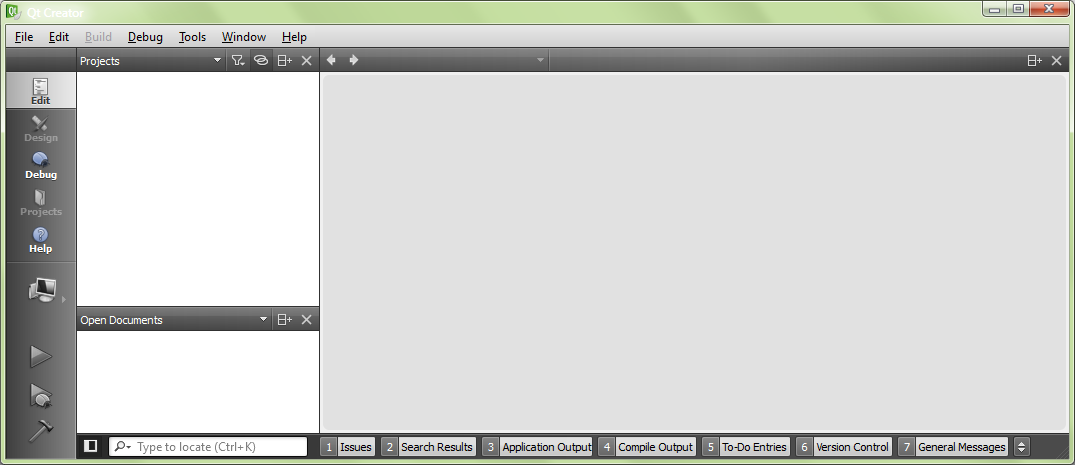
\includegraphics[width=14.5cm]{graphics/laboratory/03-qtcreator.png}
\caption{Qt Creator empty environment}\label{figure:qtcreator}
\end{figure}

Qt Creator supports big collection of features:\index{CMake}\index{Autotools}\index{QMake}
\begin{itemize}
\item multiple build systems (CMake, Autotools and QMake)
\item syntax highlighting for more than one hundred programming languages
\item auto-completion for variables, functions and macros (see \autoref{figure:qtcreatorauto})
\item consistent look on every supported operating system
\item many plugins
\item refactoring facilities
\item tools for debugging
\item cooperation with Android SDK
\item dynamic keyboard shortcuts
\item integrated Qt help system (see \autoref{figure:qtcreatorhelpfull})
\item context-aware help (see \autoref{figure:qtcreatorhelp})
\item support for simultaneously installed Qt frameworks
\item integrated Qt Designer for \fdocabbrevref{GUI} design
\item sharing source code via online services
\item many more\ldots
\end{itemize}

\begin{figure}[ht]
\centering
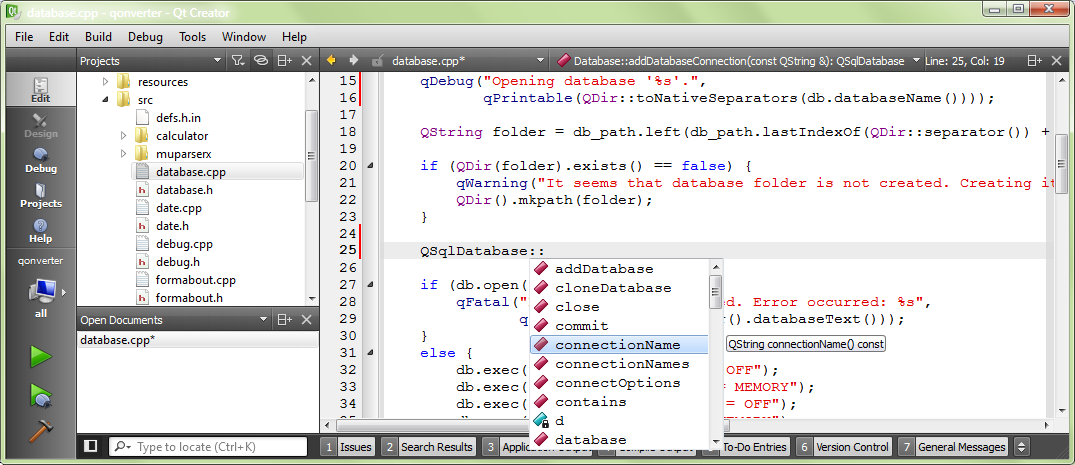
\includegraphics[width=14.5cm]{graphics/laboratory/04-qtcreator-auto.png}
\caption{Qt Creator auto-completion}\label{figure:qtcreatorauto}
\end{figure}

\begin{figure}[ht]
\centering
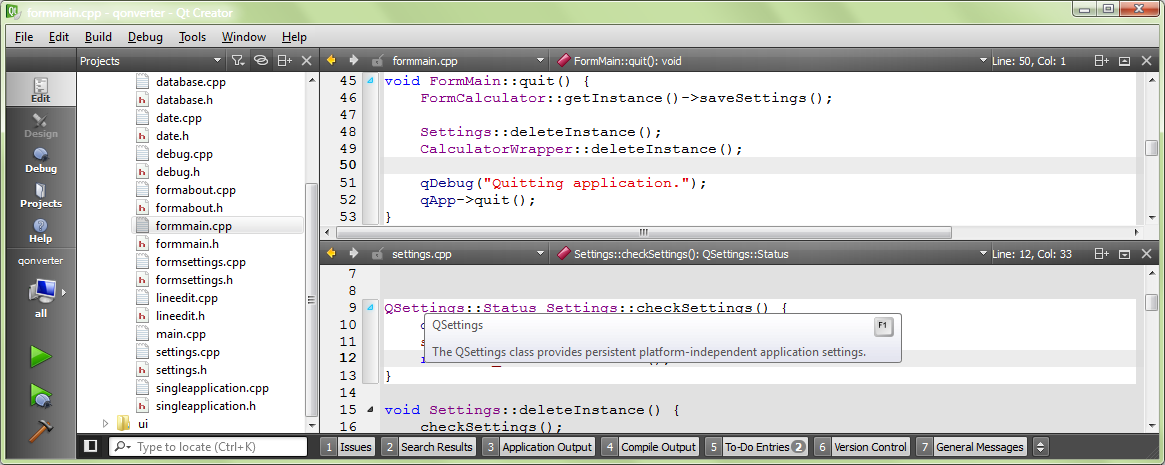
\includegraphics[width=14.5cm]{graphics/laboratory/05-qtcreator-help.png}
\caption{Qt Creator context-aware help}\label{figure:qtcreatorhelp}
\end{figure}

\begin{figure}[ht]
\centering
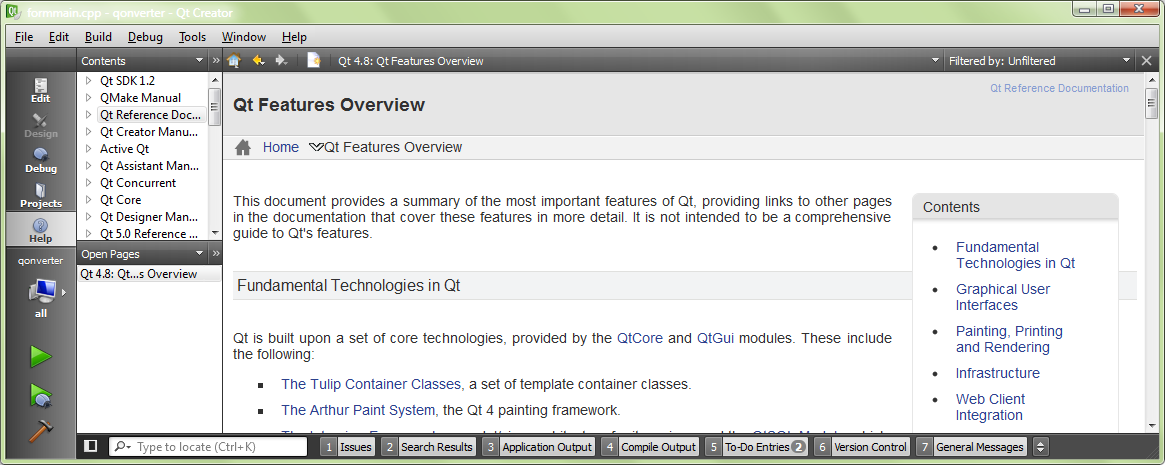
\includegraphics[width=14.5cm]{graphics/laboratory/06-qtcreator-help-full.png}
\caption{Qt Creator full reference documentation}\label{figure:qtcreatorhelpfull}
\end{figure}

\subsection{Speeding-up Qt Creator}
You can make Qt Creator less memory-hungry by disabling some unneeded plugins. You can disable plugins in\fdocinlinecode{text}{!}{About -> About Plugins...} menu. Minimal setup for desktop Qt development using CMake may look like the one in \autoref{table:plugins}.

\begin{table}[ht]
\begin{center}
\caption{Qt Creator minimal plugins setup}\label{table:plugins}
\begin{tabular}{c | c}
enabled & disabled \\
\hline
CMakeProjectManager & AutotoolsProjectManager \\
GenericProjectManager & ClassView \\
Qt4ProjectManager & CodeAnalyzer \\
QtSupport & DeviceSupport \\
CppEditor & GLSL \\
CppTools & BinEditor \\
Debugger & Bookmarks \\
Designer & ImageViewer \\
Help & Macros \\
ProjectExplorer & UpdateInfo \\
ResourceEditor & Welcome \\
CodePaster & QtQuick \\
Todo & FakeVim \\
 & HelloWorld \\
 & TaskList \\
 & VersionControl 
\end{tabular}
\end{center}
\end{table}

\section{Qt Designer}
Qt Designer\index{Qt Designer} (see \autoref{figure:designer}) is a tool for user interface design. It is standalone application which is integrated into Qt Creator too.

\begin{figure}[ht]
\centering
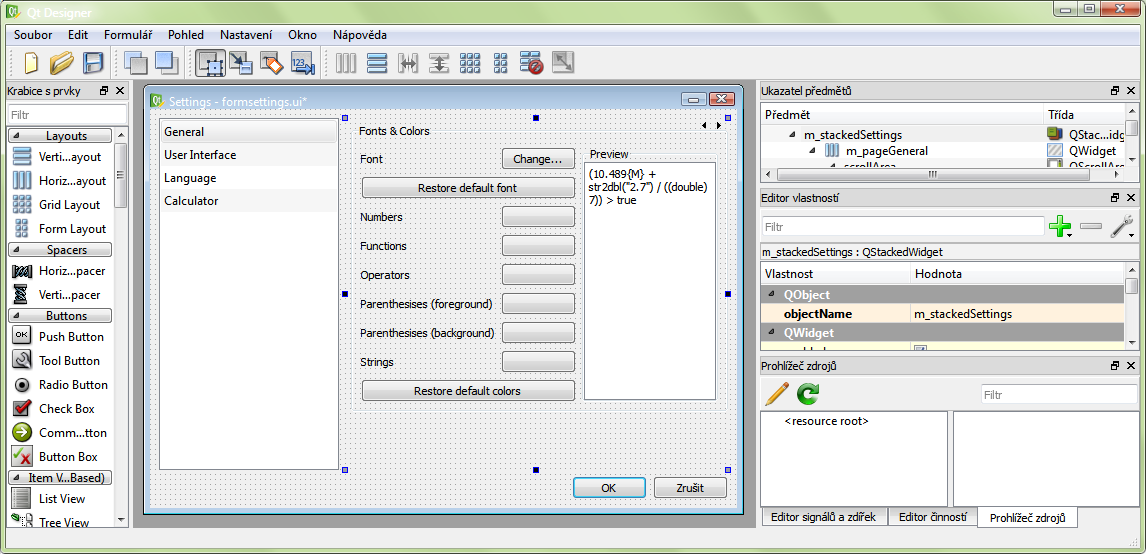
\includegraphics[width=14.5cm]{graphics/laboratory/07-designer.png}
\caption{Qt Designer environment}\label{figure:designer}
\end{figure}

\section{Tools and chains}
Qt Creator supports multiple compilers and multiple Qt libraries installed side by side. You can choose any installed compiler or Qt library to build your projects. Qt Creator uses special terminology for groups of compilers and Qt libraries called \textit{kits}. Kit (see typical kit setup in \autoref{figure:kit}) is virtual container for one compiler and one specific Qt library (for example Qt 5 library). Moreover, kit specifies primary debugger and and other stuff needed to compile your projects. Kit (or \textit{toolchain}) says what is used to compile your project. You can manage compilers and Qt versions in\fdocinlinecode{text}{!}{Build & Run} section of Qt Creator settings dialog.

\begin{figure}[ht]
\centering
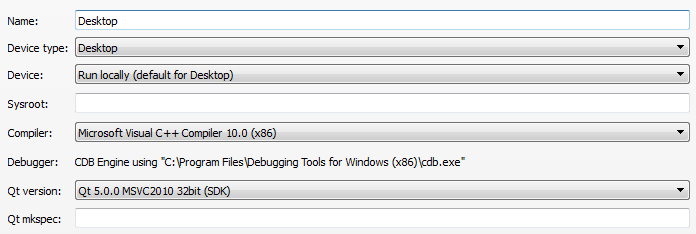
\includegraphics[width=11cm]{graphics/laboratory/08-qtcreator-kits.png}
\caption{Qt Creator kit setup}\label{figure:kit}
\end{figure}

\section{Code conventions}
Writing working application isn't, by far, enough in Qt world. Qt itself is huge library and rules are more important here than everywhere. These rules we talk about apply primarily to our source code. Code \textbf{must} be self-descriptive. This can be achieved by following certain code conventions. We are talking here about source code \enquote{typography}.\footnote{You should assure yourself you have some base to build on before you proceed. If certainty is not solid, then take a look at \citep[p.~40-77]{mcconnell:codecomplete}.}

\subsection{What are conventions?}
Programming can be very difficult job sometimes. That's why programmers do need to make their work easier. Conventions are tools to achieve that. It's always useful to know what certain source code does simply by taking a brief look at it. If this happens, then code is written well, it is readable, understandable and it's actually joy to browse it.

Let's compare source code to formatted text (\eg  text of a book). Good books do have their content formatted so that reader can read it smoothly and comfortably. It is supplemented with pictures, tables, charts and diagrams. Text itself is separated into paragraphs (usually one paragraph per idea), which can have indented first lines or can be separated by vertical white space. In addition, important words can be \textcolor{purple}{highlighted} with color or \emph{emphasised} alternatively. You can disagree with claims in this paragraph but these claims can be summed up into one thing called \emph{style}\index{style}. Your disagreement signs that there are many various styles. Some apply to books, other ones to cars. Styles are not perfect. If majority of interested people likes these adjustments (\eg visual adjustments of source code), then we call these adjustments a \emph{conventions}\index{convention}. Everything (almost) can have its style and conventions. Style makes things usable, predictable. Style 
is good.

Good programmer has to realise he produces source code not for him but for other programmers in a community or in a team. Aware programmer produces code styled the way a team (or a community) likes, not the way that he wants.

\subsection{Applying Qt conventions}
Compare \autoref{listing:badstyle} and \autoref{listing:goodstyle}. Just a brief look can advise you what is meant by code readability.
\begin{fdoccode}{cpp}{listing:badstyle}{Bad code style}
#ifndef CAR_H
#define CAR_H

#include <QtCore/QDebug>


class Car {
    private:
		unsigned int NumberOfWheels;
    public:
		Car(int w);
		void showMeThisParticularCar();
    private:
		bool owner;
};
#endif // CAR_H
\end{fdoccode}

\begin{fdoccode}{cpp}{listing:goodstyle}{Good code style}
#ifndef CAR_H
#define CAR_H


class Car {
    public:
		// Creates new car.
		Car(int number_of_wheels, bool has_owner = true);

		// Displays information about this car.
		void showCar();

    private:
		int m_numberOfWheels; // Stores count of wheels of this car.
		bool m_hasOwner; // True if this cas is owned by someone.
};

#endif // CAR_H
\end{fdoccode}

There are considerable differences between these two code fragments. Conventions importance is not probably obvious because of code length but it will grow rapidly with regard to code complexity and length. We should examine lines of \autoref{listing:goodstyle} now.

\subsection{Elements of good Qt code style}
Base for \autoref{listing:goodstyle} is sample application in\fdocinlinecode{text}{!}{sources/laboratory/06-good-car}. Let's explore both file\fdocinlinecode{text}{!}{sources/laboratory/06-good-car/car.h} and\fdocinlinecode{text}{!}{sources/laboratory/06-good-car/car.cpp}.

\subsubsection*{File car.h}
Using two blank lines between header file last\fdocinlinecode{cpp}{!}{#define} macro and class declaration beginning is generally good habit. Some programmers use just one blank line, it's a matter of taste.
\begin{lstlisting}[firstnumber=1,language=cpp]
#ifndef CAR_H
#define CAR_H


class Car {
\end{lstlisting}
Blank-lining is good in many constructs of \cpp language. One blank line should appear before each class section except the very first section.
\begin{lstlisting}[firstnumber=5,language=cpp]
class Car {
    public:
\end{lstlisting}
Comment\index{code comment} your code. Comments are essential part of source code. Always comment parts of code which are not straightforward. Uncommented code buys you ticket to hell.
\begin{lstlisting}[firstnumber=7,language=cpp]
	// Creates new car.
\end{lstlisting}
Use lower-cased names for variables in functions (methods) with undersore as delimiter for words in a variable name. Boolean variables should include verb in its name.
\begin{lstlisting}[firstnumber=8,language=cpp]
	Car(int number_of_wheels, bool has_owner = true);
\end{lstlisting}
Note that method should contain verb in its name because method always \enquote{does} something. Sometimes, single verb as name is pretty enough to describe what method does or how it works. Use Camel notation\index{notations!Camel} for methods. In Camel notation, all words in a compound (except first word) begin with upper-case letter and are not separated by spaces or any other character.
\begin{lstlisting}[firstnumber=11,language=cpp]
	void showCar();
\end{lstlisting}
Use Hungarian notation\index{notations!Hungarian} for data members of each and every class. In Hungarian notation, all variable names have prefix which signals data type or purpose of the variable. It is recommended to delimite prefixes by underscore character. Members prefixed with\fdocinlinecode{cpp}{!}{m_} are simply instance data members, while members starting with\fdocinlinecode{cpp}{!}{s_} are static data members of a class. Use this customized Hungarian notation along with Camel notation.
\begin{lstlisting}[firstnumber=14,language=cpp]
	int m_numberOfWheels; // Signs count of wheels of this car.
	bool m_hasOwner; // Does this car have an owner?
\end{lstlisting}

\subsubsection*{File car.cpp}
Include Qt header\index{headers} files first, since they may include system-based header files, so that you have less inclusions in your source after all. Your own header files should be included as last ones. Leave two blank lines (sometimes one blank line is enough) between headers inclusions and rest of source code.
\begin{lstlisting}[firstnumber=1,language=cpp]
#include <QDebug>

#include "car.h"


Car::Car(int number_of_wheels, bool has_owner) {
\end{lstlisting}
Don't use\fdocinlinecode{cpp}{!}{s_} or\fdocinlinecode{cpp}{!}{m_} prefixes for variables with method scope (the ones declared inside method) because those are not data members.
\begin{lstlisting}[firstnumber=6,language=cpp]
    m_numberOfWheels = number_of_wheels;
    m_hasOwner = has_owner;
\end{lstlisting}

\begin{fdocextra}
Inclusion of header files is a matter that should attract our attention. It is \textbf{highly} recommended to avoid typing used Qt module into header file path, for example writing\fdocinlinecode{cpp}{!}{#include <QtCore/QDebug>} is not good idea.

\fdocinlinecode{cpp}{!}{QDebug} class could be removed from QtCore module and moved into some newly forged one in the future.\footnotemark{} This code won't work with that hypothetical Qt build. Include Qt stuff in a simpler way instead, for example\fdocinlinecode{cpp}{!}{#include <QDebug>} is much better. Don't include entire Qt modules either. Reason is the same. Moreover, you could include parts of a module you would never use in your application.
\end{fdocextra}
\footnotetext{That has actually happened with Qt 5 release. Module QtWidgets was created and some classes from QtGui were moved into it.}

As we said, code style is unique for each and every programmer in some detail. If you program an application, try to stop from time to time and imagine you're someone who sees that piece of code for the first time and try to think about goal of that code. Or even better, send your code to someone else for review.